\chapter{RGB-D图像的获取与融合}
\label{chap:rgbd}
RGB-D图像是所设计的三维物体识别算法的输入,其质量对算法结果有着至关重要的影响,以此获取高质量的RGB-D图像也十分重要。本章首先分析了3D相机的现状,然后详细介绍了选取的RGB-D相机的原理和标定流程,并且针对其缺点提出了对偶RGB-D相机结构,最后通过实验证明了对偶RGB-D相机可以获取更高质量的RGB-D图像。

\section{3D相机现状与分析}
3D相机能够获取相机到物体表面每一点的距离,从而感知物体的形状和距离,近几年3D成像技术的应用越来越多,如用于体感游戏的Kinect\cite{kinect},Google的Project Tango\cite{tango},以及Apple公司的iPhone X前置摄像头的人脸识别。

目前市面上的3D相机要么价格昂贵,要么精度低下,很难找到一款性价比较高的3D相机。
\begin{table}[ht]
  \centering
  \begin{tabular}{cccc}
    \toprule
    品牌&价格&精度&速度 \\
    \midrule
    SICK&大于30万&高&很慢 \\
    Enshape&大于30万&高&较快 \\
    Ensenso&约10万&较高&较快 \\
    Realsense&约1.5千&中等&快 \\
    Kinect V2&约1.5千&低&快\\
    \bottomrule
  \end{tabular}
  \caption{市面上主要3D相机价格和性能}
  \label{tab:3d_camera}
\end{table}
\begin{figure}[ht]
  \centering
  \subfloat[SICK]{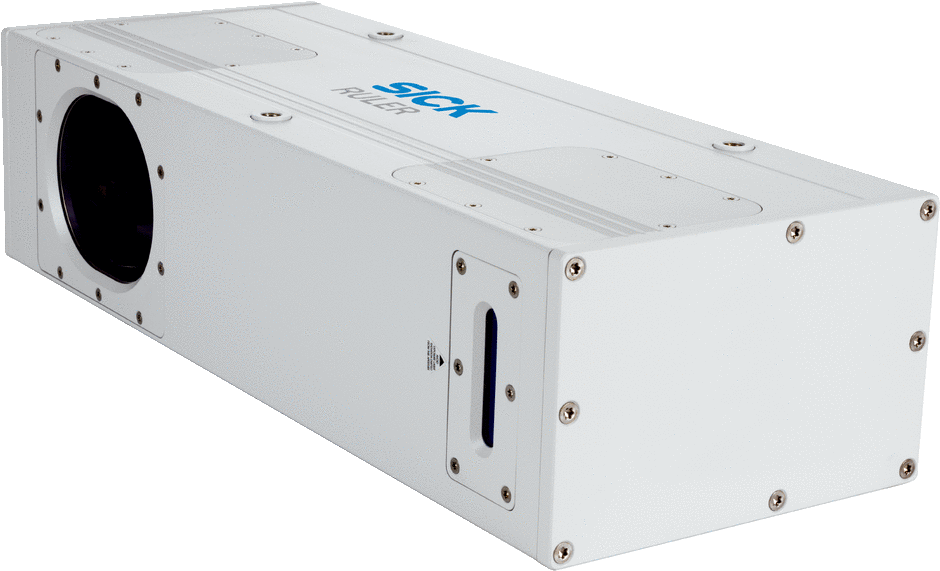
\includegraphics[width=3cm]{sick}}
  \subfloat[Enshape]{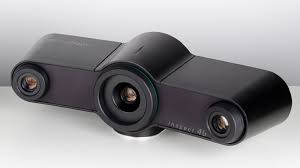
\includegraphics[width=3cm]{enshape}}
  \subfloat[Ensenso]{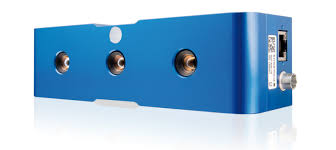
\includegraphics[width=3cm]{ensenso}}
  \subfloat[Realsense]{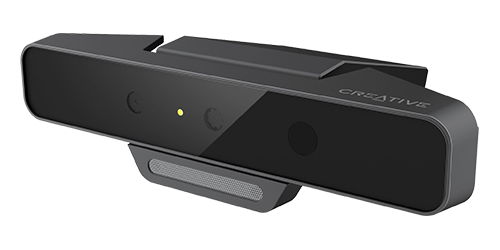
\includegraphics[width=3cm]{realsense}}
  \subfloat[Kinect V2]{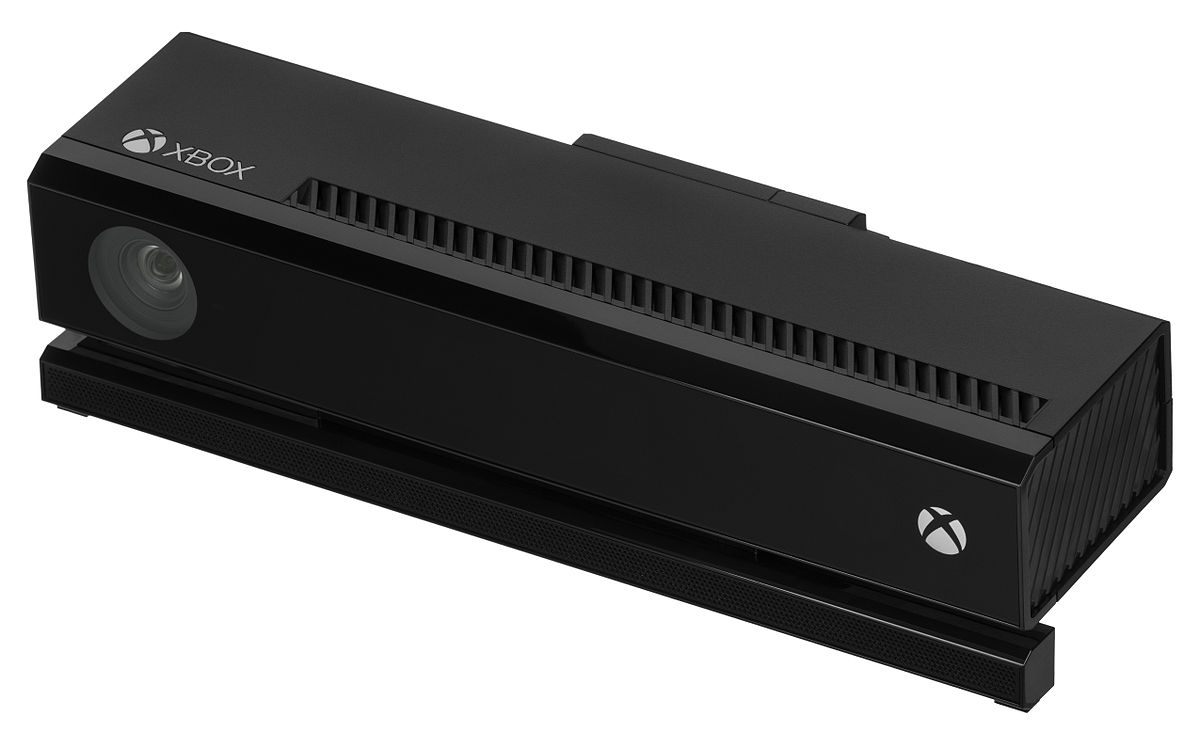
\includegraphics[width=3cm]{kinect}}
  \caption{市面上主要3D相机}
  \label{fig:3d_camera}
\end{figure}
如表\ref{tab:3d_camera}和图\ref{fig:3d_camera}所示,列举了一些市面上较为常见的3D相机,从表中可以发现很多精度高的3D相机价格及其昂贵,并且采集速度很慢,价格低的3D相机精度有相对较低。出于实际应用考虑,我们需要相机的采集速度相对较快,再加上成本上的限制,最终选择了精度中等、采集速度较快、价格较为便宜的Realsense系列相机。


\section{RGB-D相机}
\subsection{RGB-D相机原理与结构}
RGB-D相机获取深度的原理大致可以分为三种:
\begin{itemize}
\item Structure Light
\item Time of Flight(ToF)
\item Stereo
\end{itemize}

% @improve: 加些原理图?
Structure Light获取深度信息的原理是通过激光发射器投射带有特定编码的结构光到物体表面后,由IR Camera采集,根据采集到的光信号量的变化来计算物体的深度。举一个形象的例子,将手电筒照向墙面,手电筒离墙面越远,墙面上所形成的光斑的直径就越大,所以可以通过光斑的直径来计算手电筒距离墙面的距离。ToF获取深度信息的原理是通过专有的传感器捕捉红外光发射到接收的飞行时间来计算物体的深度。Stereo是通过双摄像头拍摄物体,再通过特征点匹配,根据三角测量原理来计算物体的深度。

三种原理的深度相机各有其特点,采用Structure Light原理的深度相机一般精度比较高,但景深比较短并且受光线影响比较大,适合室内场景;ToF原理的深度相机获取深度图的精度和分辨率一般都比较低,但帧率高,并且具有一定的抗光照性能;Stereo获取深度精度适中,帧率相对来说较低,并且需要较强的计算性能,但抗光照能力强,适合室外场景。

本文所使用的RGB-D相机是Intel的Realsense SR300相机,SR300采用的结构光的原理获取深度\footnote{此后所提到的RGB-D相机均指与SR300相机类似的采用结构光原理获取深度的RGB-D相机},其内部结构如图\ref{fig:sr300}所示。
\begin{figure}[!ht]
  \centering
  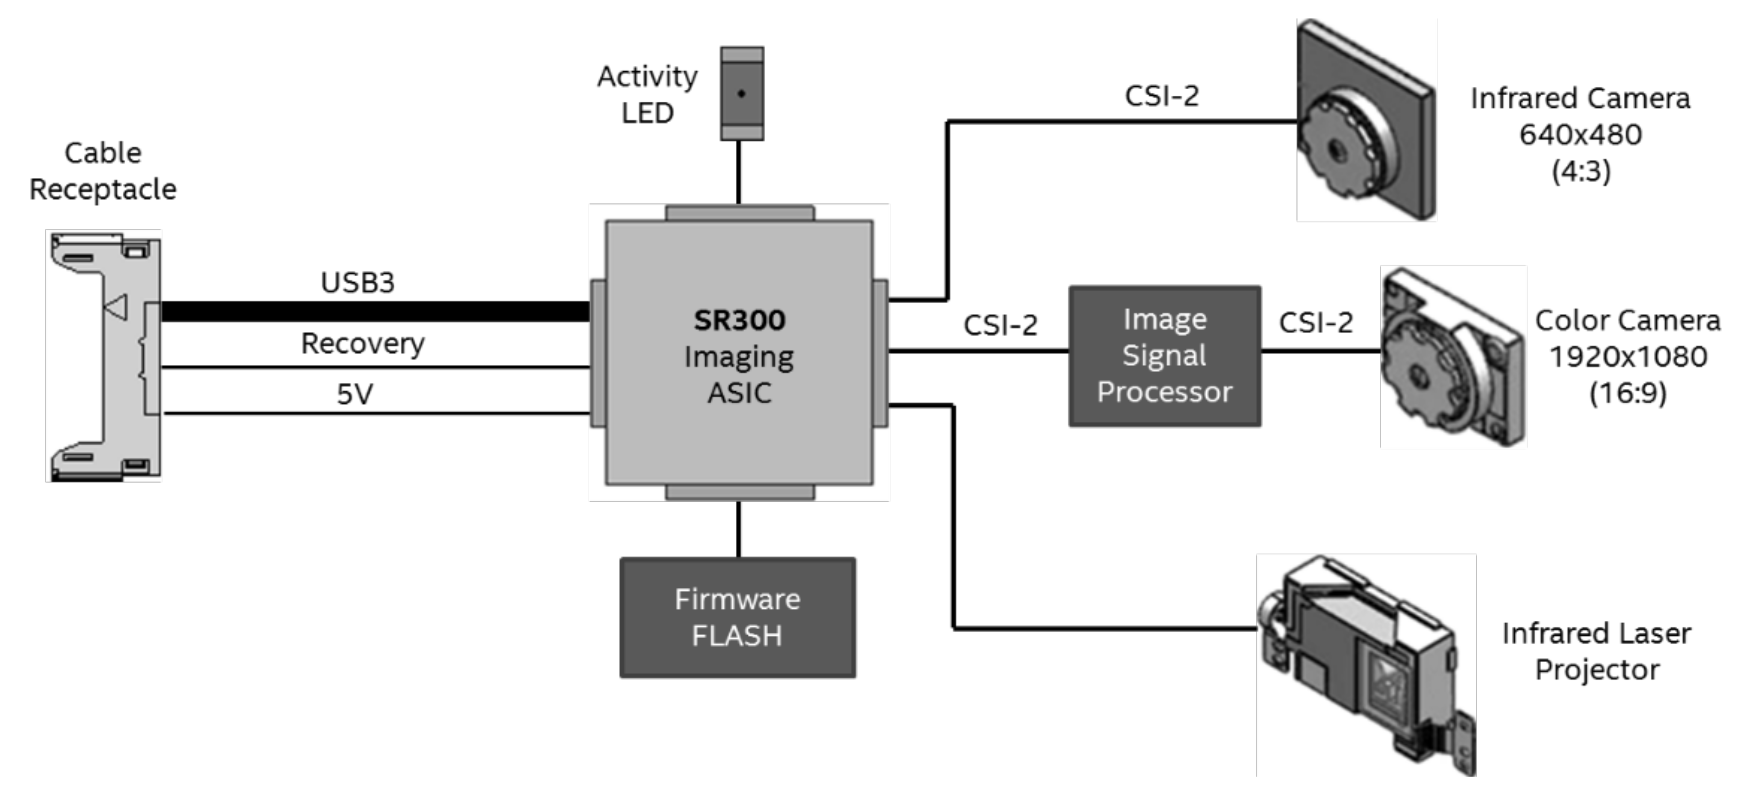
\includegraphics[width=12cm]{sr300}
  \caption{Realsense SR300内部结构图}
  \label{fig:sr300}
\end{figure}
从图\ref{fig:sr300}可以看出,SR300内部的传感器主要有彩色摄像头(Color Camera)、红外激光发射器(Infrared Laser Projector)和红外摄像头(Infrared Camera)。Color Camera是1920×1080像素的普通针孔摄像头,用来获取彩色图像;Infrared Laser Projector和Infrared Camera用来获取深度图像或者红外成像图,两种成像流程如图\ref{fig:capture_flow}所示。
\begin{figure}[!ht]
  \centering
  \subfloat[Depth Video Data Flow]{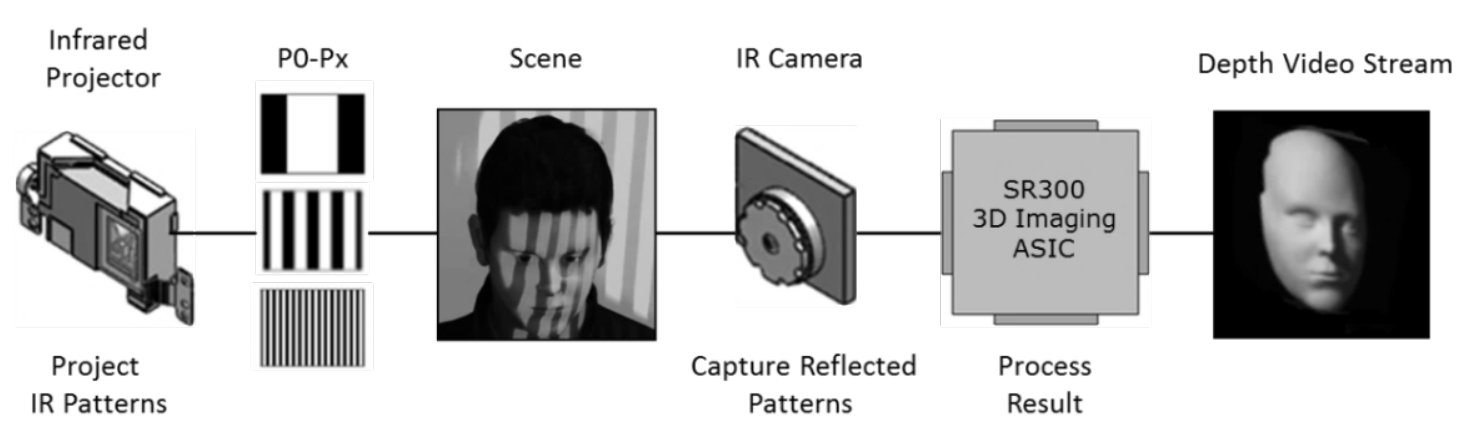
\includegraphics[width=12cm]{depth_flow}}
  \vfill
  \subfloat[IR Video Data Flow]{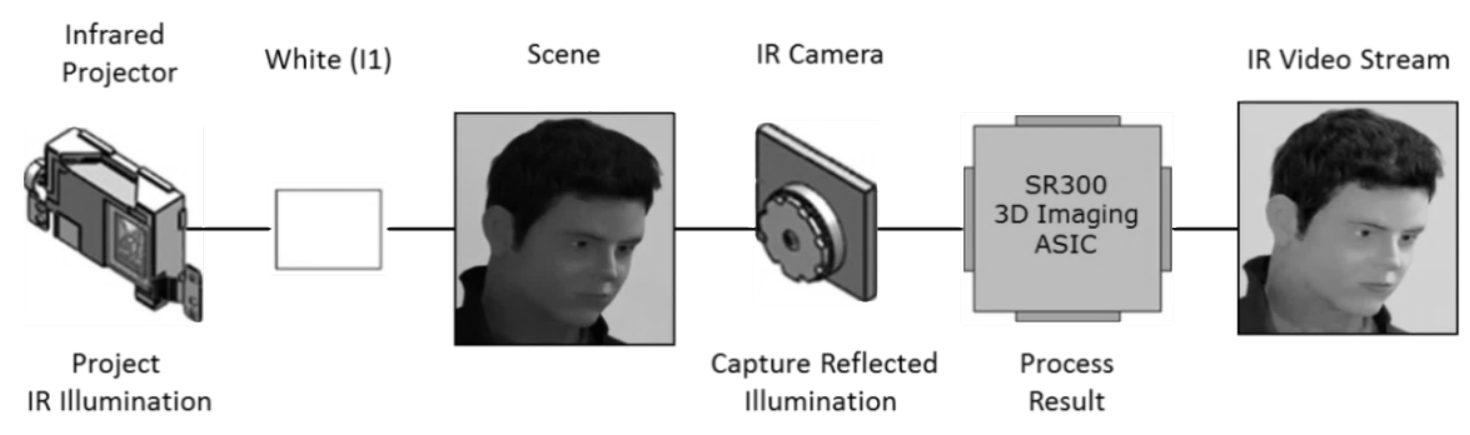
\includegraphics[width=12cm]{ir_flow}}
  \caption{Realsense SR300深度成像流程}
  \label{fig:capture_flow}
\end{figure}
其中当Infrared Laser Projector投射带有编码的结构光时,Infrared Camera可以获取深度图;当投射不带编码的红外光时,Infrared Camera可以获取红外成像图。正常使用时,往往设置Infrared Laser Projector投射带有编码的结构光来获取深度信息。因此,从RGB-D相机的使用来看,可以忽略其内部具体结构,将其看成由一个彩色摄像头和一个深度摄像头构成,其中彩色摄像获取彩色(RGB)信息,深度摄像头获取深度(depth)信息。

\subsection{RGB-D相机的数学模型}
% @improve: actually, color and depth's distortion model are different.
\begin{figure}[!ht]
  \centering
  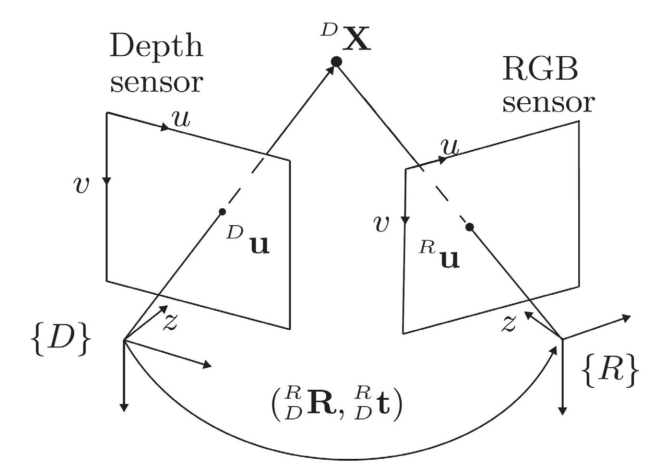
\includegraphics[width=8cm]{rgbd_model}
  \caption{RGB-D相机模型}
  \label{fig:rgbd_model}
  % @improve: draw the figure use tikz
\end{figure}
图\ref{fig:rgbd_model}展示了本文所使用的RGB-D相机的基本物理模型,其中彩色摄像头和深度摄像头都使用了针孔(pin-hole)相机模型\cite{Heikkila2000}。
先考虑普通针孔相机的模型,相机图像坐标系下一点$\bm{u}:=[u,v]^T$,对应的三维世界中的一点在相机坐标系下表示为$\bm{X}:=[x,y,z]^T$。根据针孔相机模型有:
\begin{equation}
  \label{eq:cam_model}
  z\bm{\tilde{u}} = \bm{K}\bm{X}
\end{equation}
其中$\bm{\tilde{u}}$表示$\bm{u}$的齐次变换形式,彩色相机的内参矩阵$\bm{K}$的定义如下:
\begin{equation}
  \bm{K} := \left[
    \begin{array}{ccc}
      f_u&0&u_0 \\
      0&f_v&v_0 \\
      0&0&1
    \end{array}
  \right]
\end{equation}
其中$f_u$和$f_v$分别表示彩色相机在图像坐标轴上的焦距(以像素为单位),$u_0$和$v_0$表示彩色相机光心在图像平面的投影中心。

公式\ref{eq:cam_model}还未考虑镜头的畸变,为了提高相机的精度,现引入径向畸变(radial distortion)和切向畸变(tangential distortion):
\begin{itemize}
\item 径向畸变是由相机透镜的不完善和表面曲率存在误差造成的,径向畸变的数学模型可以表示为:
  \begin{equation}
    \label{eq:radial}
    \left\{
      \begin{array}{ccc}
        \hat{x}&=&\bar{x}(1 + k_1r^2 + k_2r^4 + k_3r^6)\\
        \hat{y}&=&\bar{y}(1 + k_1r^2 + k_2r^4 + k_3r^6)\\
      \end{array}
    \right.
  \end{equation}
  其中
  \begin{align}
    \bar{x} =& x/z\\
    \bar{y} =& y/z\\
    r  =& \sqrt{\bar{x}^2 + \bar{y}^2}
  \end{align}
  $\bar{x}$,$\bar{y}$表示点$\bm{X}$在归一化平面上的坐标,$\hat{x}$,$\hat{y}$表示修正径向畸变后的的坐标,$k_1$,$k_2$,$k_3$表示径向畸变的参数。
\item 切向畸变是由于相机透镜与图像平面不平行造成的,其数字模型可以表示为:
  \begin{equation}
    \label{eq:trang}
    \left\{
      \begin{array}{ccc}
        \hat{x}&=&\bar{x} + (2p_1\bar{x}\bar{y} + p_2(r^2 + 2\bar{x}^2))\\
        \hat{y}&=&\bar{y} + (p_1(r^2 + 2\bar{y}^2) + 2p_2\bar{x}\bar{y})\\
      \end{array}
    \right.
  \end{equation}
  其中$p_1$,$p_2$是切向畸变的参数。
\item 结合公式\ref{eq:radial}和\ref{eq:trang}可以得到修正径向畸变和切向畸变的Brown–Conrady模型\cite{Brown1966}:
  \begin{equation}
    \label{eq:dist}
    \left\{
      \begin{array}{ccc}
        \hat{x}&=&\bar{x}(1 + k_1r^2 + k_2r^4 + k_3r^6) + (2p_1\bar{x}\bar{y} + p_2(r^2 + 2\bar{x}^2))\\
        \hat{y}&=&\bar{y}(1 + k_1r^2 + k_2r^4 + k_3r^6) + (p_1(r^2 + 2\bar{y}^2) + 2p_2\bar{x}\bar{y})\\
      \end{array}
    \right.
  \end{equation}
\end{itemize}
通过以上分析,根据公式\ref{eq:cam_model}和\ref{eq:dist}可以推导出带有畸变的针孔相机模型:
\begin{equation}
  \label{eq:dist_cam_model}
  \left\{
    \begin{array}{ccc}
      u&=&f_u(\bar{x}(1 + k_1r^2 + k_2r^4 + k_3r^6) + (2p_1\bar{x}\bar{y} + p_2(r^2 + 2\bar{x}^2))) + u_0\\
      v&=&f_v(\bar{y}(1 + k_1r^2 + k_2r^4 + k_3r^6) + (p_1(r^2 + 2\bar{y}^2) + 2p_2\bar{x}\bar{y})) + v_0
    \end{array}
  \right.
\end{equation}
为方便起见,记$\bm{d}:=[k_1,k_2,p_1,p_2,k_3]^T$,定义函数
\begin{equation}
  f_{undist}(\bm{d}, \bm{X}):=\left[
    \begin{array}{ccc}
      \bar{x}(1 + k_1r^2 + k_2r^4 + k_3r^6) + (2p_1\bar{x}\bar{y} + p_2(r^2 + 2\bar{x}^2))\\
      \bar{y}(1 + k_1r^2 + k_2r^4 + k_3r^6) + (p_1(r^2 + 2\bar{y}^2) + 2p_2\bar{x}\bar{y})\\
    \end{array}
  \right]
\end{equation}
\begin{equation}
  \tilde{f}_{undist}(\bm{d}, \bm{X}):=\left[
    \begin{array}{c}
      f_{undist}(\bm{d}, \bm{X})\\
      1
    \end{array}
  \right]
\end{equation}
则公式\ref{eq:dist_cam_model}可简化为:
\begin{equation}
  \tilde{\bm{u}} = \bm{K}\cdot \tilde{f}_{undist}(\bm{d}, \bm{X})
\end{equation}
其中需要标定的参数有相机内参矩阵$\bm{K}$(包含未知参数$f_u$,$f_v$,$u_0$,$v_0$)以及畸变参数$\bm{d}$(包含未知参数$k_1$,$k_2$,$p_1$,$p_2$,$k_3$),共9个参数。

明确了针孔相机的数学模型后,很容易推出SR300的相机模型:
\begin{equation}
  \label{eq:rgbd_cam_model}
  \left\{
    \begin{array}{ccc}
      \tensor*[^R]{\tilde{\bm{u}}}{}&=&\tensor*[^R]{\bm{K}}{}\cdot \tilde{f}_{undist}(\tensor*[^R]{\bm{d}}{},\tensor*[^R]{\bm{X}}{})\\
      \tensor*[^D]{\tilde{\bm{u}}}{}&=&\tensor*[^D]{\bm{K}}{}\cdot \tilde{f}_{undist}(\tensor*[^D]{\bm{d}}{},\tensor*[^D]{\bm{X}}{})\\
      \tensor*[^R]{\bm{X}}{} &=& \tensor*[^R_D]{\,\bm{R}}{}\tensor*[^D]{\bm{X}}{} + \tensor*[^R_D]{\,\bm{t}}{}
    \end{array}
  \right.
\end{equation}
其中左上标$\{R\}$表示SR300相机中的彩色相机(RGB),$\{D\}$表示SR300相机中的深度相机(Depth),$\tensor*[^R_D]{\,\bm{R}}{}$和$\tensor*[^R_D]{\,\bm{t}}{}$表示了彩色相机坐标系和深度相机坐标系之间的齐次变换关系。

\subsection{RGB-D相机的标定流程}
\label{sec:rgb-d_calibration}
根据上文所述的RGB-D相机的结构及数学模型,RGB-D相机的标定主要涉及到彩色摄像头内参和畸变的标定,深度摄像头内参和畸变的标定,以及彩色摄像头和深度摄像头之间位姿变换的标定。由于RGB-D相机是一种较为新颖的相机,所以市面上基本上没有较为成熟通用的标定RGB-D相机的方法以及对应的工具。因此本文针对所使用的Realsense SR300相机,设计了一套标定方法。

根据公式\ref{eq:rgbd_cam_model}可知相机需要标定的参数有彩色相机内参和畸变参数9个,深度相机内参和畸变参数9个,彩色相机和深度相机之间的位姿关系6个,一共24个参数。一起标定这24个参数理论上是相当困难的,考虑到普通针孔相机的标定技术已经相当成熟(如张正友的棋盘格标定\cite{Zhang2002},以及RGB-D相机中彩色相机和深度相机的解耦性,因此所设计的标定方法分为三步:
\begin{enumerate}[Step 1]
\item 标定彩色相机内参以及畸变参数
\item 标定深度相机内参以及畸变参数
\item 标定彩色相机和深度相机之间的齐次变换关系
\end{enumerate}

步骤1标定彩色相机内参以及畸变参数相对来说比较简单,主要参考文献\cite{Zhang2002},但所使用的标定板是不对称圆盘标定板(Asymmetrical Circle Board),如图\ref{fig:circle_board}是$4\times 11$的不对称圆盘标定板。
\begin{figure}[!ht]
  \centering
  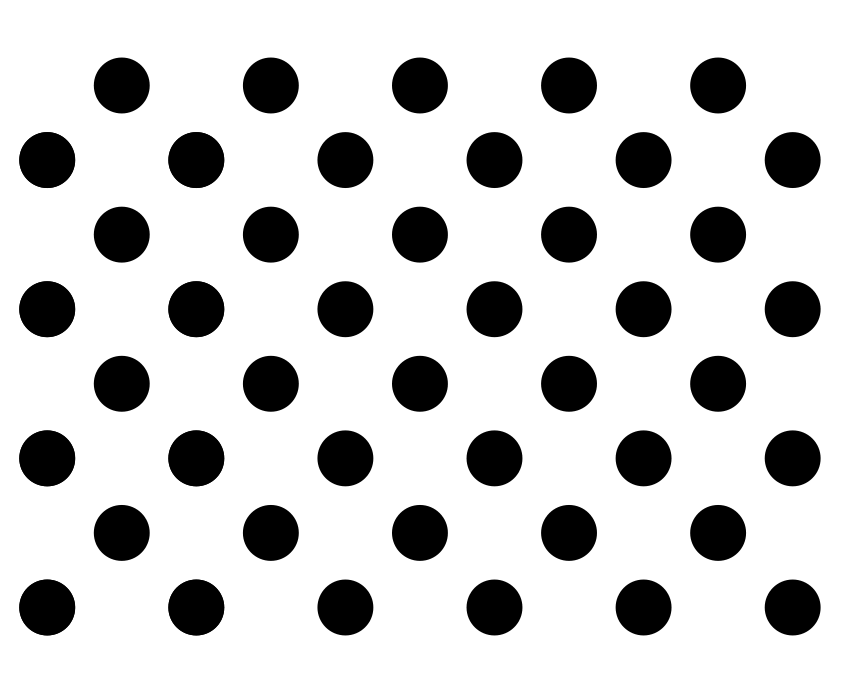
\includegraphics[width=10cm]{circle_board}
  \caption{Asymmetrical Circle Board}
  \label{fig:circle_board}
\end{figure}
使用圆盘标定板而非棋盘格标定板的原因是圆盘相对于棋盘格有更高的检测精度,在某些情况下可以达到0.1到0.01像素的亚像素精度,当然代价是相比计算棋盘格的角点,计算椭圆(圆形经过投影变换后退化为椭圆)的中心会涉及到较为复杂的数学运算,这也是为什么工业上大多使用圆盘作为标定板的原因。

步骤2标定深度相机内参以及畸变参数的方法和步骤1类似,区别在于深度相机并不能直接获得颜色信息,因此也不能直接检测图\ref{fig:circle_board}所示的标定板。但是,幸运的是,根据前文所述的SR300深度相机的原理,其本质上也是个普通的针孔相机,只不过在其镜头上加上了滤波片,可以认为其只对红外光成像。因此,只要使用图\ref{fig:capture_flow}中的红外成像模式获取红外成像图,在红外成像图上检测标定板。如图\ref{fig:circle_on_ir}所示,在红外成像图中检测出了标定板。
\begin{figure}[!ht]
  \centering
  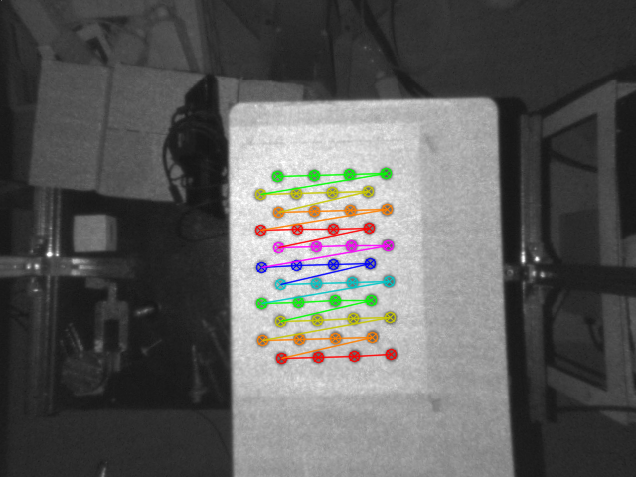
\includegraphics[width=12cm]{circle_on_ir}
  \caption{红外成像图中检测标定板}
  \label{fig:circle_on_ir}
\end{figure}

步骤3标定彩色相机和深度相机之间的齐次变换关系需要依赖于步骤1和步骤2中标定出的彩色相机和深度相机的内参和畸变参数,具体做法是将标定板放在彩色相机和深度相机下,使彩色相机和深度相机能够同时检测到标定板,然后分别根据各自的内参和畸变参数计算出标定板的位姿$\tensor*[^R_B]{\bm{H}}{}$和$\tensor*[^D_B]{\bm{H}}{}$,其中$\tensor*[^R_B]{\bm{H}}{}$是$4\times 4$的齐次变换矩阵,表示标定板在彩色相机坐标系下的位姿,也是彩色相机坐标系变换到标定板坐标系的齐次变换矩阵;$\tensor*[^D_B]{\bm{H}}{}$也是$4\times 4$的齐次变换矩阵,表示标定板在深度相机坐标系下的位姿,也是深度相机坐标系变换到标定板坐标系的齐次变换矩阵。从而所要求的彩色相机坐标系变换到深度相机坐标系的齐次变换矩阵为:
\begin{equation}
  \tensor*[^R_D]{\bm{H}}{} = \tensor*[^R_B]{\bm{H}}{}\tensor*[^D_B]{\bm{H}}{^{-1}}
\end{equation}
其中
\begin{equation}
  \tensor*[^R_D]{\bm{H}}{} := \left[
    \begin{array}{cc}
      \tensor*[^R_D]{\bm{R}}{}& \tensor*[^R_D]{\bm{t}}{}\\
      \bm{0}_{1\times 3}&1
    \end{array}
\right]
\end{equation}
当然,实际标定时,往往会采取多组$\tensor*[^R_B]{\bm{H}}{}$和$\tensor*[^D_B]{\bm{H}}{}$来提高标定的精度。

\section{对偶RGB-D相机}
使用SR300相机时,发现相机在某些情况下,对一些反光的物体的深度图有严重的缺失,具体如图\ref{fig:depth_missing}所示。
\begin{figure}[!ht]
  \centering
  \subfloat[彩色图]{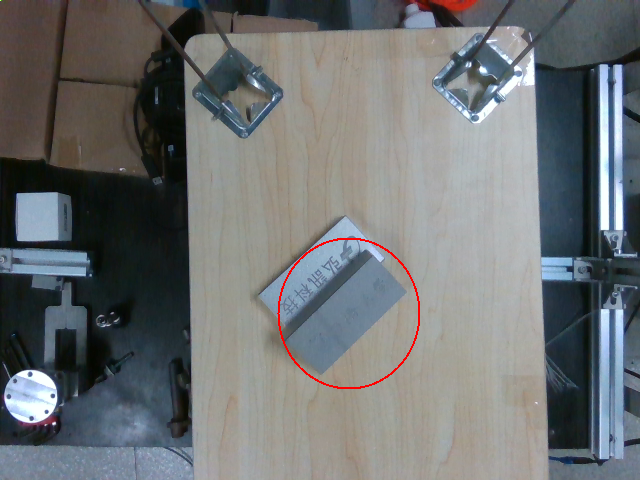
\includegraphics[width=7cm]{left_color}}
  \hfill
  \subfloat[深度图]{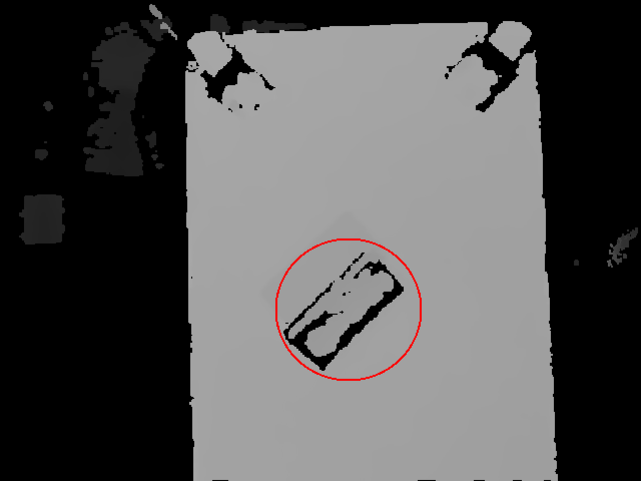
\includegraphics[width=7cm]{left_depth}}
  \caption{SR300采集的物体深度信息部分缺失情况下的深度图}
  \label{fig:depth_missing}
\end{figure}
经过实验,发现这种缺失情况的出现和拍摄的角度以及光线有关,因此本文提出一种组合相机对偶RGB-D相机(Dual RGB-D Camera)。

\subsection{对偶RGB-D相机原理与结构}
对偶RGB-D相机在原RGB-D相机的基础上,通过增加一个与原相机呈180度夹角的RGB-D相机构成,实际物理结构如图\ref{fig:dual_rgbd}所示。
\begin{figure}[!ht]
  \centering
  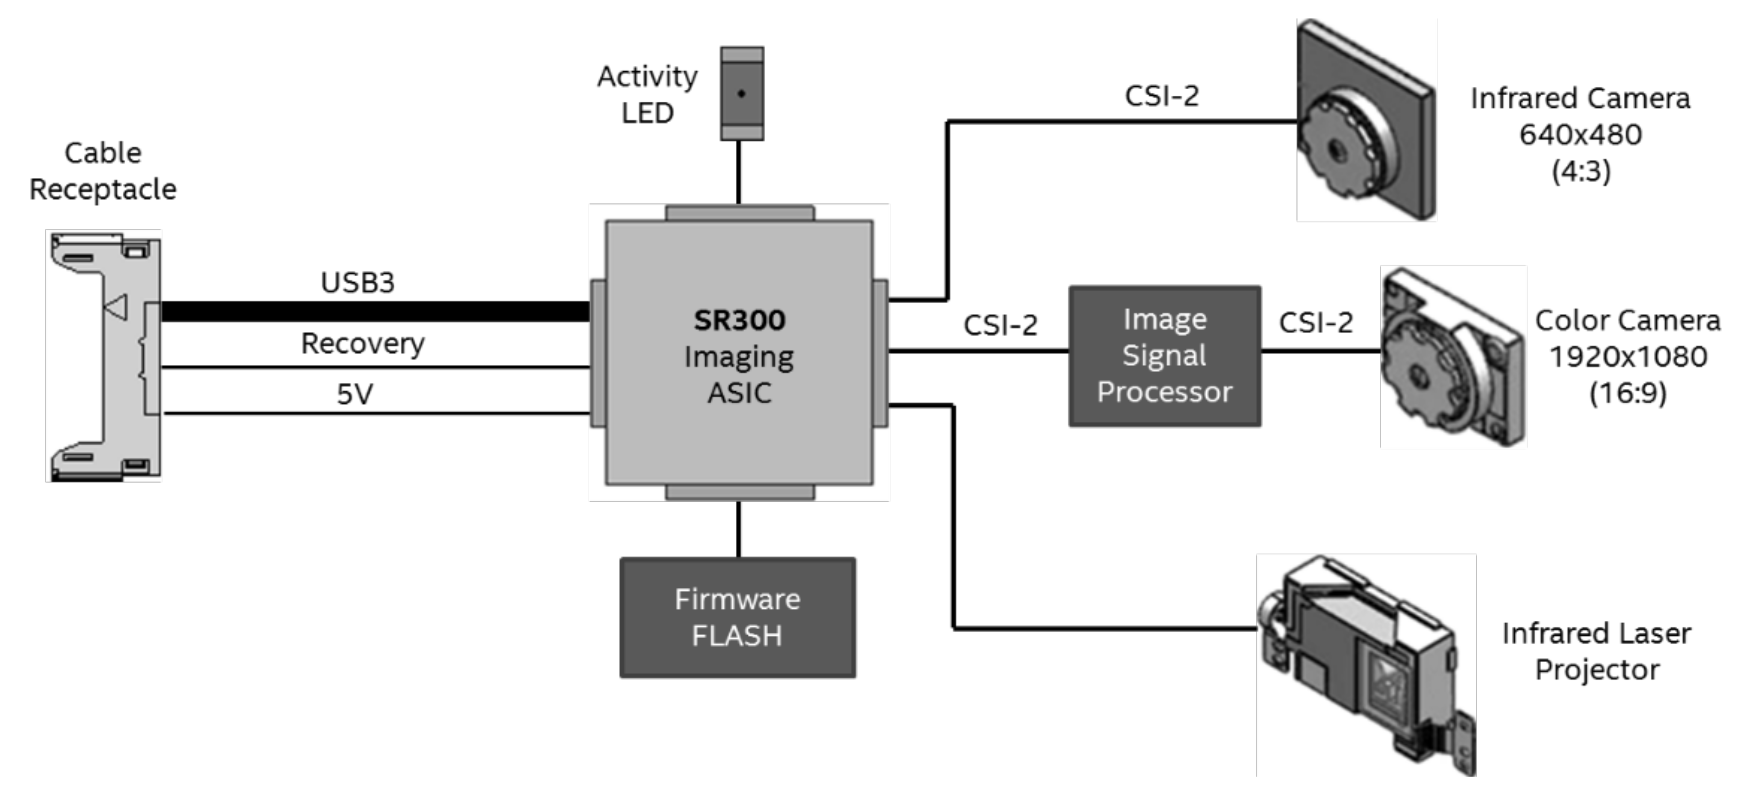
\includegraphics[width=6cm]{dual_rgbd}
  \caption{对偶RGB-D相机实际物理结构}
  \label{fig:dual_rgbd}
\end{figure}

对于对偶RGB-D相机,当其中一个相机深度图出现严重缺失时,另外一个相机的深度图往往不会在相同的地方深度信息出现严重的缺失,如图\ref{fig:dual_rgbd_depth}所示\footnote{实际下相机采集的图像与上相机采集的图像相差了180度,为了方便起见,都将下相机采集的图像旋转了180度}
,有效的避免了单个RGB-D相机某些情况下深度信息严重缺失的情况。
\begin{figure}[!ht]
  \centering
  \subfloat[上相机采集的深度图]{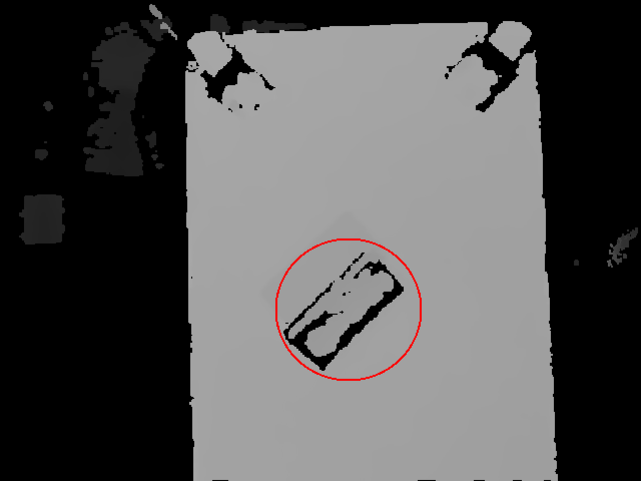
\includegraphics[width=7cm]{left_depth}}
  \hfill
  \subfloat[下相机采集的深度图]{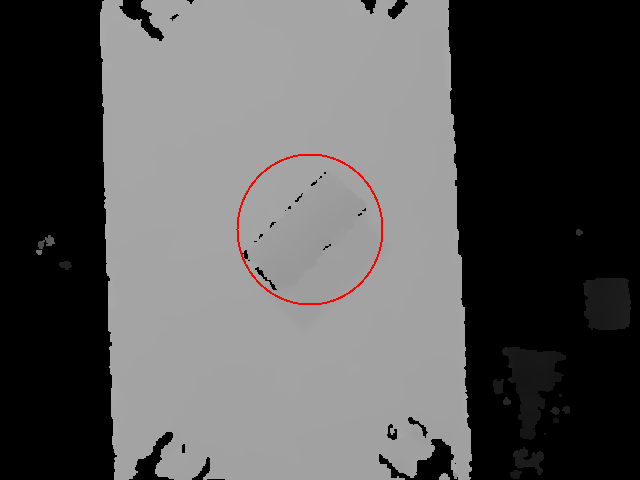
\includegraphics[width=7cm, angle=180, origin=c]{right_depth}}
  \caption{对偶RGB-D相机采集的左右两张深度图}
  \label{fig:dual_rgbd_depth}
\end{figure}

除此之外,对偶RGB-D相机还可以利用两个相机的彩色图构成双目,生成第三张深度图,从而通过设计的深度的融合算法将三张深度图融合成为一张质量更高的深度图,其内部原理如图\ref{fig:dual_rgbd_struct}所示。
\begin{figure}[!ht]
  \centering
  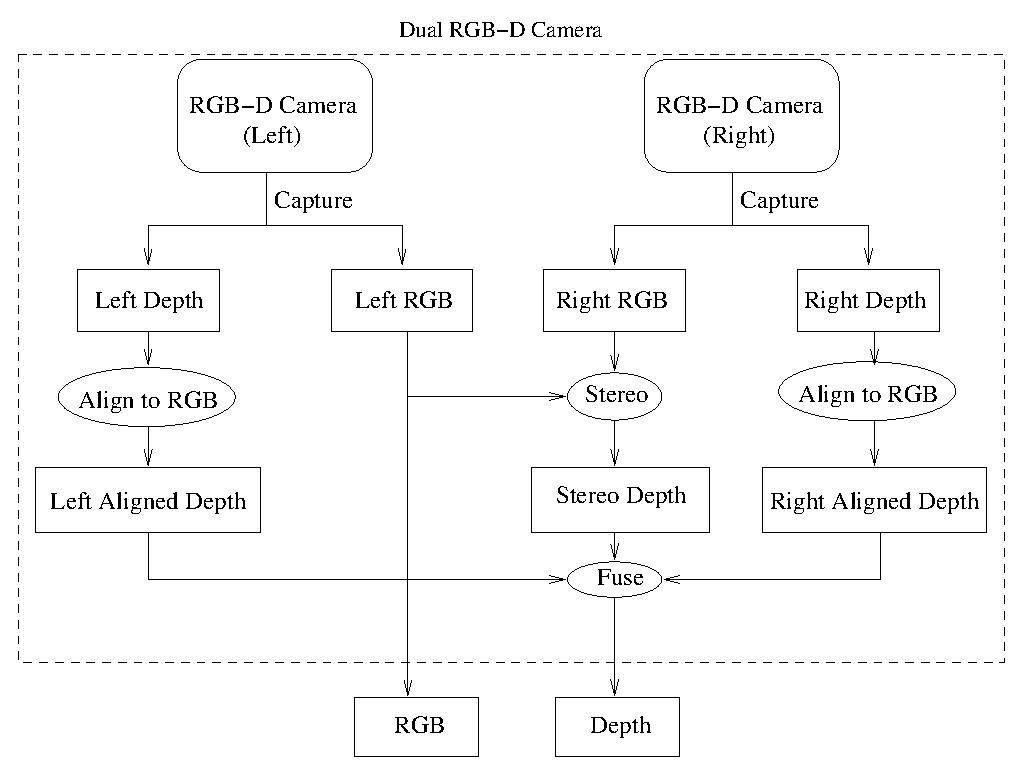
\includegraphics[width=14cm]{dual_rgbd_struct}
  \caption{对偶RGB-D相机内部原理图}
  \label{fig:dual_rgbd_struct}
\end{figure}

从外部使用来看,对偶RGB-D相机也输出一张彩色图、一张深度图。输出的彩色图就是从上相机采集到的彩色图;输出的深度图是由三张深度图融合而成,并且与输出的彩色图相对齐,对齐的意思是彩色图和深度图相同图像坐标下的颜色信息和深度信息对应的实际物理世界中相同的一点,对齐的意义在于方便后续的一些图像处理的算法。

从内部实现来看,主要涉及到三个部分:
\begin{itemize}
\item 将深度图与输出的彩色图对齐(Align to RGB)
\item 利用上相机采集的彩色图和下相机采集的彩色图,通过双目匹配算法形成一张新的深度图
\item 融合上相机对齐后的深度图、下相机对齐后的深度图和双目匹配得到的深度图
\end{itemize}
将深度图与彩色图对齐,相对来讲实现还是比较简单的,对齐深度图的具体流程如算法\ref{alg:align}所示。
\begin{algorithm}[!ht]
  \caption{Align Depth Frame}
  \label{alg:align}
  \KwIn{Raw Depth Frame $Raw\_D_{dh\times dw}$}
  \KwOut{Aligned Depth Frame $Aligned\_D_{ch\times cw}$}
  \For {p in $Aligned\_D$} {
    $p = 0$
  }
  \For {dy = 1; dy <= dh; ++dy} {
    \For {dx = 1; dx <= dw; ++dx} {
      通过深度相机内参将点$(dx, dy)$反投影到三维空间一点$\tensor*[^D]{\bm{X}}{}$\;
      坐标变换$\tensor*[^R]{\bm{X}}{} = \tensor*[^R_D]{\bm{R}}{}\tensor*[^D]{\bm{X}}{} + \tensor*[^R_D]{\bm{t}}{}$\;
      通过彩色相机内参将点$\tensor*[^R]{\bm{X}}{}$投影变换到彩色图像坐标系下一点$(cx, cy)$\;
      \If {cx in $(0, cw]$ and cy in $(0, ch]$} {
        $Aligned\_D(cx, cy) = Raw\_D(dx, dy)$\;
      }
    }
  }
\end{algorithm}
算法\ref{alg:align}主要将深度图中每个点的图像坐标利用该点的深度信息反投影变换到实际三维空间中一点,然后将该点坐标变换到彩色相机坐标系下,最后通过彩色相机的内参将该点在彩色相机坐标系下的三维坐标投影变换到彩色图像上的二维坐标。实际对齐三张深度图时,对于上相机深度图对齐到上相机彩色图,需要分别知道上相机深度相机和彩色相机的内参和畸变参数以及深度相机与彩色相机之间的齐次变换关系(通过相机标定这些参数都可以得到);双目匹配得到的深度图理论上可以有两张,一张与上相机校准后的彩色图像对齐,另一张与下相机校准后的彩色图像对齐,简单起见,选择与上相机对齐的深度图,然后通过上相机校准所使用的旋转矩阵的逆矩阵即可得到与原上相机彩色图像对齐的深度图;对齐下相机到上相机彩色图,除了要知道下相机标定的参数外,还需要知道下相机与上相机之间的齐次变换关系(通过对偶RGB-D相机的标定得到)。

利用上下相机采集到的两张彩色图获取深度信息主要分为三步:
\begin{itemize}
\item 分别对两张原始图像进行校准
\item 在校准后的两张图像上通过匹配算法得到视差图
\item 通过视差图获取深度图
\end{itemize}
对两张原始图像进行校准主要通过双目相机的标定实现,使得校准后的两张图像的极线对齐,如图\ref{fig:stereo_images}所示,
\begin{figure}[!ht]
  \centering
  \subfloat[上相机原始图像]{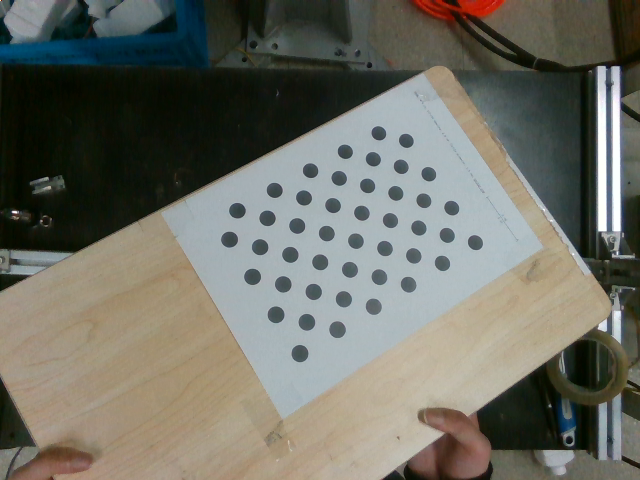
\includegraphics[width=7cm]{left_raw_image}}
  \hfill
  \subfloat[上相机校准后图像]{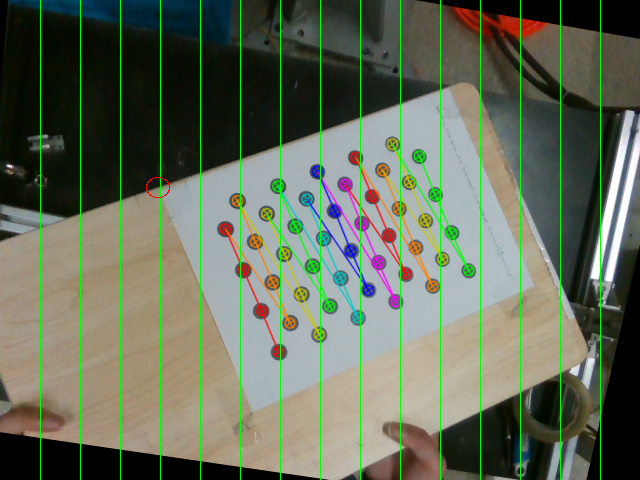
\includegraphics[width=7cm]{left_rectified_image}}
  \vfill
  \subfloat[下相机原始图像]{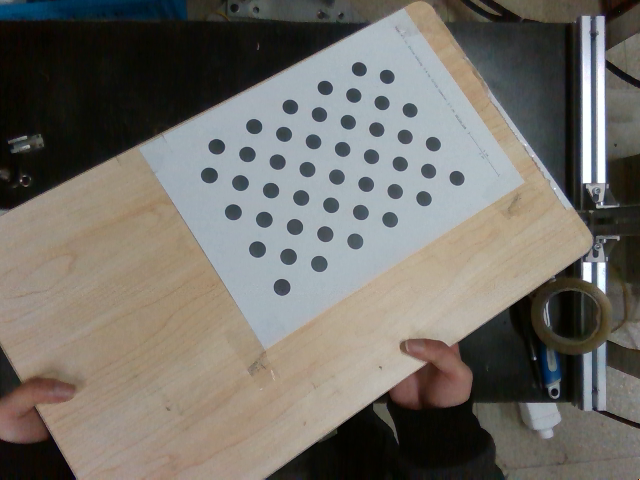
\includegraphics[width=7cm]{right_raw_image}}
  \hfill
  \subfloat[下相机校准后图像]{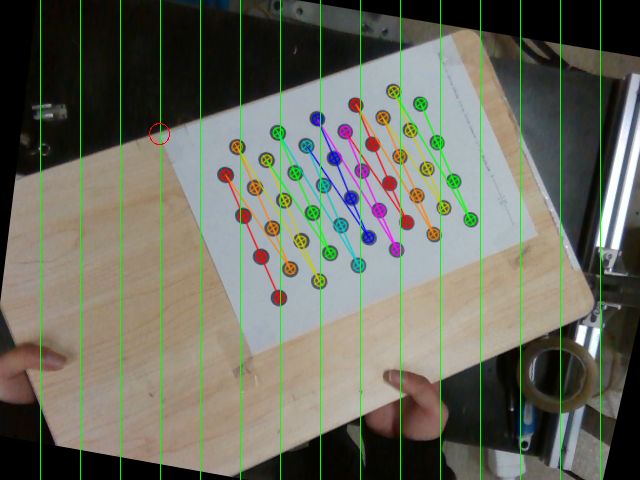
\includegraphics[width=7cm]{right_rectified_image}}
  \caption{双目相机原始图像和校准后图像}
  \label{fig:stereo_images}
\end{figure}
其中绿色的直线便是图像对齐后的部分极线,可以看出校准后的图像的对应点都分布在对齐的极线上(如图中用红色圈出的一对对应点所示),这样使得双目的匹配算法的搜索从二维缩小到了一维,只需要在极线上找对应点即可,能更快更稳定地在两张图中找到对应点。双目匹配算法使用的是ELSA算法\cite{Geiger2010},通过ELSA算法可以从两张校准后彩色图像上得到对应的视差图,视差图到深度图的变化可以通过公式\ref{eq:reprojection}得到:
\begin{equation}
  \label{eq:reprojection}
  z = \frac{\prescript{\{T,\,R\}}{}{f}B}{-(\prescript{\{T,\,R\}}{}{v_0}-\prescript{\{B,\,R\}}{}{v_0}) + \prescript{\{T,\,R\}}{}{d}}
\end{equation}
其中上标\{$T,R$\}(Top,RGB)表示上相机的RGB摄像头,\{$B,R$\}(Bottom,RGB)表示下相机的RGB摄像头,$B$表示基线长度,$\prescript{\{T,\,R\}}{}{d}$表示视差。一般地,会人为地校准过程中使得$\prescript{\{T,\,R\}}{}{v_0}-\prescript{\{B,\,R\}}{}{v_0}=0$,从而公式\ref{eq:reprojection}可以简化为:
\begin{equation}
  \label{eq:reprojection_simple}
  z = \frac{\prescript{\{T,\,R\}}{}{f}B}{\prescript{\{T,\,R\}}{}{d}}
\end{equation}

融合上相机对齐后的深度图、下相机对齐后的深度图以及双目匹配得到的深度这三张深度图的算法首先做的是分别对这三张深度图进行预处理,填补一些深度缺失的像素,因为对齐后的深度图和双目匹配得到的深度图深度信息都有细微的缺失,填补深度信息缺失的方法如算法\ref{alg:fill_hole}所示。
\begin{algorithm}[!ht]
  \caption{Fill Holes in Depth Frame}
  \label{alg:fill_hole}
  \KwIn{Depth Frame $D_{h\times w}$}
  \KwOut{Filled Depth Frame $FD_{h\times w}$}
  \For {y = 1; y <= h; ++y} {
    \For {x = 1; x <=w ; ++x} {
      \If {valid($D_{x,y}$)} {
        $FD_{x,y} = D_{x,y}$\;
      } \Else {
        $FD_{x,y}$= NAN\;
        bool leftTop = valid($D_{x-1, y-1}$) or valid($D_{x, y-1}$) or valid($D_{x-1, y}$)\;
        bool leftBottom = valid($D_{x-1, y+1}$) or valid($D_{x, y+1}$) or valid($D_{x-1, y}$)\;
        bool rightTop = valid($D_{x+1, y-1}$) or valid($D_{x, y-1}$) or valid($D_{x+1, y}$)\;
        bool rightBottom = valid($D_{x+1, y+1}$) or valid($D_{x, y+1}$) or valid($D_{x+1, y}$)\;
        \If {leftTop and leftBottom and rightTop and rightBottom} {
          validPoints = \{\}\;
          \For {dy = -1; dy <=1; ++dy} {
            \For {dx = -1; dx <=1; ++dx} {
              \If {valid($D_{dx, dy}$)} {
                push back $D_{x, y}$ to validPoints\;
              }
            }
          }
          \If {max(validPoints) - min(validPoints) < 0.05} {
            $FD_{x,y}$= mean(validPoints)\;
          }
        }
      }
    }
  }
\end{algorithm}
算法\ref{alg:fill_hole}主要实现对于深度缺失的点,将检查其周围的深度信息,当其四个角上都有有效的深度信息时,并且周围有效深度信息的极值小于一定阈值时,会用周围有效深度信息的均值填充该缺失的点。实际的效果如图\ref{fig:fill_hole}所示。
\begin{figure}[!ht]
  \centering
  \subfloat[填补前]{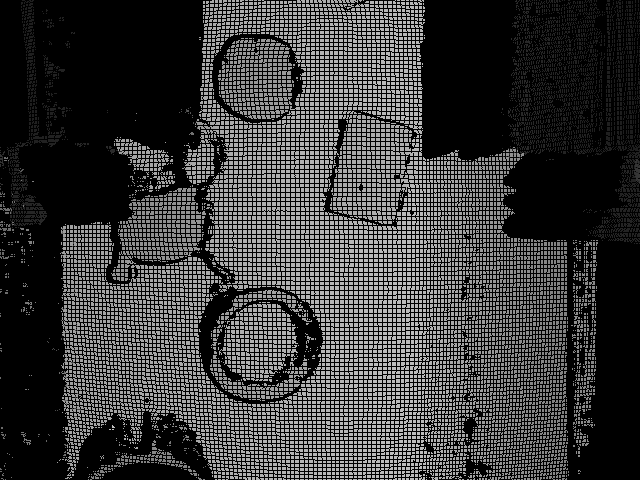
\includegraphics[width=6cm]{fillhole1}}
    \hskip1.5cm
  \subfloat[填补后]{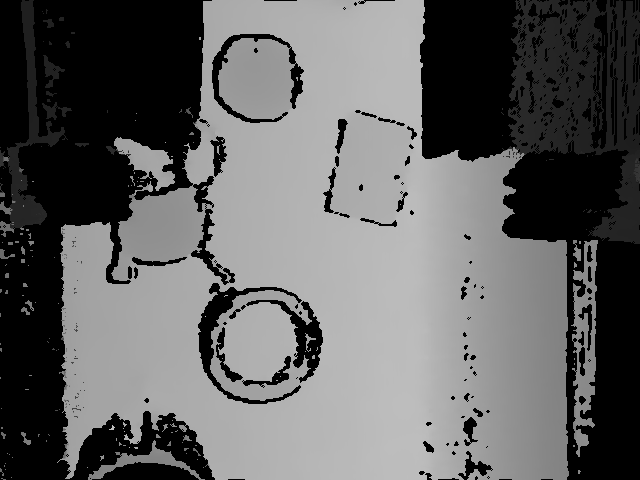
\includegraphics[width=6cm]{fillhole2}}
  \caption{填补深度信息缺失算法效果图}
  \label{fig:fill_hole}
\end{figure}
分别对深度图进行预处理后,将会对三张深度图进行线性叠加得到最终的深度图,基本叠加的公式如\ref{eq:linear}所示。
\begin{equation}
  \label{eq:linear}
  d_{fuse} = \frac{w_1d_{left} + w_2d_{right}+w_3d_{stereo}}{w_1+w_2+w_3}
\end{equation}
其中$w_1,w_2,w_3$分别表示上相机深度、下相机深度以及双目匹配深度的权重,SR300相机得到深度的精度比双目计算得到的深度要高,所以实际使用时$w_1,w_2$要比$w_3$大许多。融合三张深度图的理论相对简单,但实际上,三张深度图的深度信息并非都会永远有效,因此根据实际情况实际的融合算法如\ref{alg:fuse}所示。
\begin{algorithm}[!ht]
  \caption{Fuse Depth Frames}
  \label{alg:fuse}
  \KwIn{leftDepth, rightDepth, stereoDepth}
  \KwOut{fuseDepth}
  Initialize w1,w2,w3\;
  \For {(d1,d2,d3,d4) in (leftDepth, rightDepth, stereoDepth, fuseDepth)} {
    validDepth = [], validWeight = []\;
    \For {i = 1 to 3} {
      \If {di is valid} {
        push back di to validDepth, wi to validWeight\;
      }
    }
    \If {size of validDepth == 0} {
      d4 = NAN\;
    } \ElseIf {size of validDepth == 1} {
      d4 = validDepth[1]\;
    } \ElseIf {size of validDepth == 2 } {
      \If {extremum of validDepth < 0.03} {
        d4 = validDepth $\cdot$ validWeight / sum of validWeight\;
      } \Else {
        d4 = NAN\;
      }
    } \Else {
      mediumDepth = medium(validDepth)\;
      d4 = 0, sum = 0\;
      \For {(d,w) in (validDepth, validWeight)} {
        \If {abs(d-mediumDepth) < 0.03} {
          d4 += d*w\;
          sum += w\;
        }
      }
      \If {sum > 0} {
        d4 = d4 / sum\;
      } \Else {
        d4 = NAN\;
      }
    }
  }
\end{algorithm}
算法\ref{alg:fuse}不仅考虑了深度缺失的情况,对于深度信息差值过大的情况也进行了处理。实际处理的效果如图\ref{fig:fuse}所示。
\begin{figure}[!ht]
  \centering
  \subfloat[Upper depth]{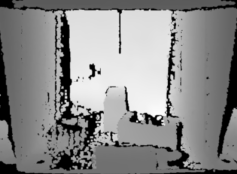
\includegraphics[width=3.5cm]{upper-depth}}
  \hskip2pt
  \subfloat[Lower depth]{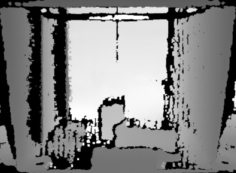
\includegraphics[width=3.5cm]{lower-depth}}
  \hskip2pt
  \subfloat[Stereo depth]{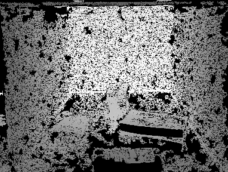
\includegraphics[width=3.4cm]{stereo-depth}}
  \hskip2pt
  \subfloat[Fuse depth]{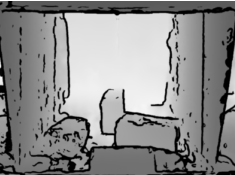
\includegraphics[width=3.5cm]{fuse-depth}}
  \caption{深度融合算法效果图}
  \label{fig:fuse}
\end{figure}

\subsection{对偶RGB-D相机的标定流程}
对偶RGB-D相机的标定流程可以分为三步:
\begin{enumerate}[Step 1]
\item 分别标定好单个RGB-D相机
\item 标定出两个彩色相机之间的齐次变换关系
\item 标定出矫正彩色图像的旋转矩阵以及矫正后图像的投影矩阵
\end{enumerate}
单个RGB-D相机的标定在\ref{sec:rgb-d_calibration}小节中已经详细叙述过了,分别标定完单个RGB-D相机后,后面的步骤其实就等价于双目标定了。双目的几何结构如图\ref{fig:stereo}所示,
\begin{figure}[!ht]
  \centering
  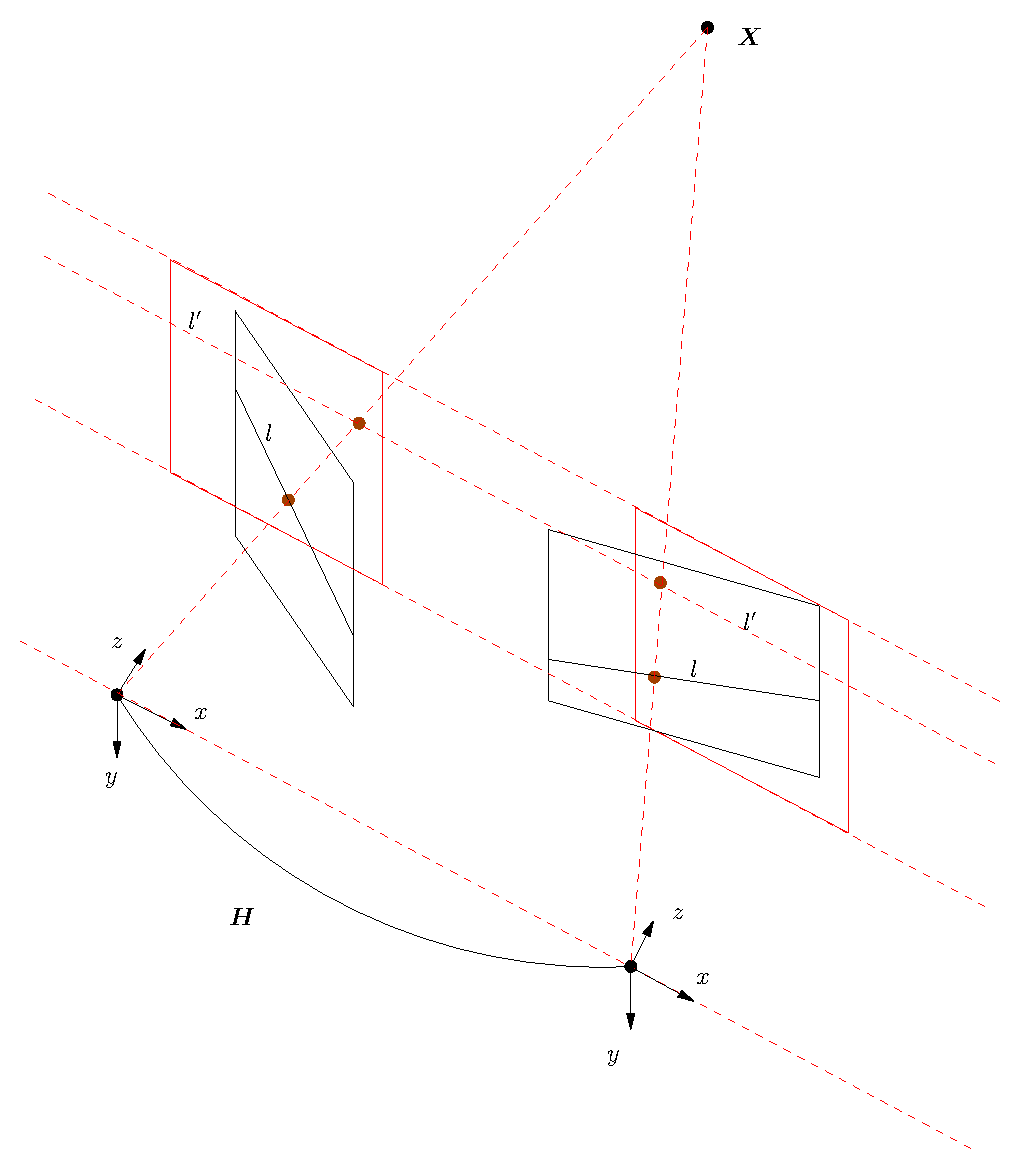
\includegraphics[width=14cm]{stereo}
  \caption{双目几何结构}
  \label{fig:stereo}
\end{figure}
标定出两个彩色相机之间的齐次变换关系,即图\ref{fig:stereo}中的$H$,简单地可以通过8点法\cite{Sur2008}先求出基础矩阵(Fundamental Matrix)$F$,即所谓的“弱标定”,然后根据相机的内参矩阵可求得本质矩阵(Essential Matrix)$E$:
\begin{equation}
  E = K^{T}FK'
\end{equation}
其中$K$和$K'$分别是两个相机的内参矩阵。求得本质矩阵后可以通过奇异值分解求得齐次变换矩阵的旋转矩阵$R$和平移向量$T$:
\begin{equation}
  \left\{\begin{array}{ccc}
    E &=& U\Sigma V^T \\
    R &=& U\bm{R}_Z^T(\frac{\pi}{2})V^T \\
    \left[T\right]_{\times} &=& U\bm{R}_Z^T(\frac{\pi}{2})\Sigma U^T
  \end{array}
  \right.
\end{equation}
其中$\bm{R}_Z(\theta)$表示绕$Z$轴旋转$\theta$角的旋转矩阵,$\left[T\right]_{\times}$的定义如下:
\begin{equation}
  \left[T\right]_{\times} = \left[
    \begin{array}{ccc}
      0&-T_z&T_y\\
      T_z&0&-T_x \\
      -T_y&T_x&0
    \end{array}
  \right]
\end{equation}
矫正彩色图像的旋转矩阵会将图\ref{fig:stereo}中黑色线框的图像平面变换到红色线框的图像平面上,使得对应点在两张图像的同一条极线上。矫正彩色图像的旋转矩阵的计算参考文献\cite{Loop2001},此步标定完最终可以得到:
\begin{itemize}
\item 两个相机的矫正旋转矩阵$R_1$,$R_2$
\item 两个矫正坐标系下的投影矩阵$P_1$,$P_2$
\item 主相机\footnote{另外一个相机的投影变换矩阵也可以得到,但没有必要。}的投影变换矩阵$Q$
\end{itemize}
其中
\begin{equation}
  Q = \left[
    \begin{array}{cccc}
      1&0&0&-u_0 \\
       0&1&0&-v_0 \\
       0&0&0&f \\
       0&0&1/B&0
    \end{array}
    \right]
\end{equation}
包含了公式\ref{eq:reprojection_simple}由视差计算深度的所有参数。

\section{深度图质量测试实验}
RGB-D相机相对于彩色图我们更关心其深度图的质量,因此设计实验测试了所采用的SR300相机深度图的质量以及改进的由两个SR300相机所组成的对偶RGB-D相机深度图的质量。通过实验,主要考察相机采集的深度在不同距离下的填充率、精度和噪声这三个指标。实验器材除了测试所用的相机,还需要沿固定方向运动的导轨,以及固定在导轨上的平板,相机通过采集平板上的深度信息来计算填充率、精度和噪声这三个指标。实际实验时,由于实验室没有沿固定方向运动的导轨,但是有六轴机械臂,所以将平板固定在机械臂末端,然后通过机械臂示教器控制机械臂末端沿固定方向移动,并且移动的距离可在示教器上读出,整个实验装置如图\ref{fig:depth_exp_env}所示。
\begin{figure}
  \centering
  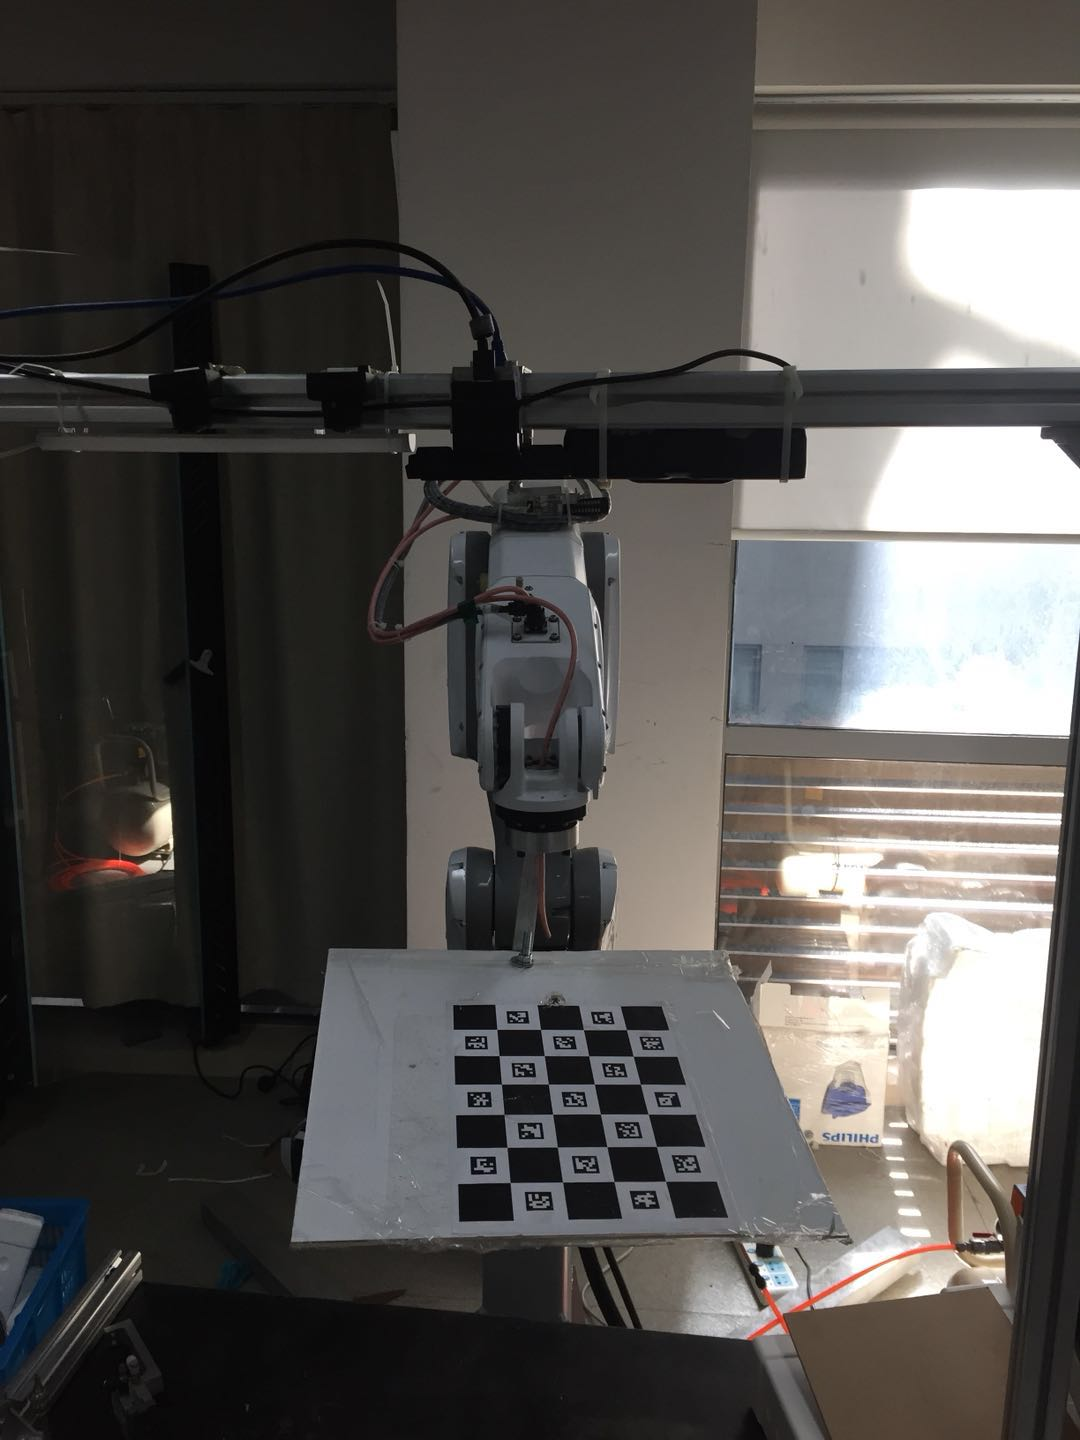
\includegraphics[width=8cm]{depth-exp-env}
  \caption{深度测试实验装置}
  \label{fig:depth_exp_env}
\end{figure}

\subsection{实验流程}
实验流程示意图如图\ref{fig:depth_exp_steps}所示,
\begin{figure}[ht]
  \centering
  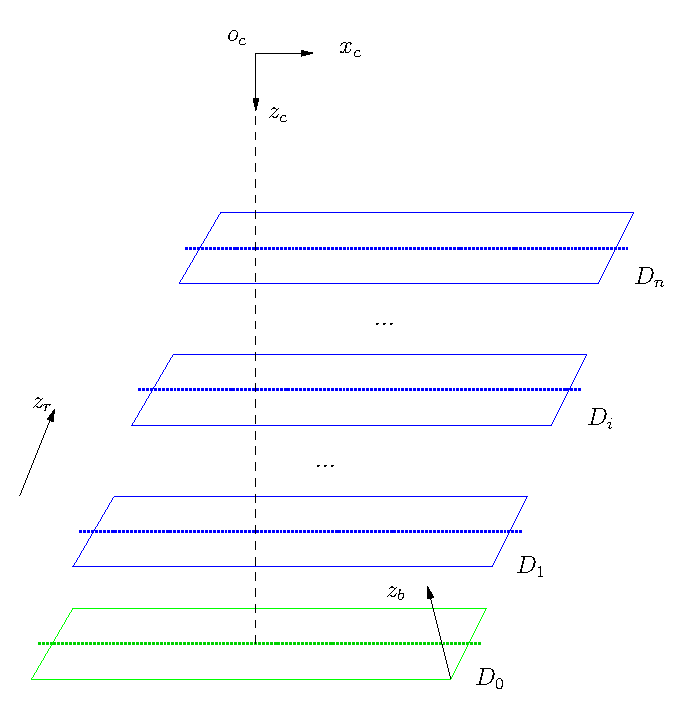
\includegraphics[]{depth_exp_steps}
  \caption{实验流程图}
  \label{fig:depth_exp_steps}
\end{figure}
其中$z_c$是相机坐标系的$z$轴方向,$z_r$是机械臂末端运动方向,也是平板运动方向,$z_b$是垂直于平板的方向,$D_i:=\{d_1,d_2,…,d_{n_i}\}$是相机采集到平板的深度信息。具体实验步骤如下:
\begin{itemize}
\item 固定机械臂和相机,通过手眼标定(具体见\ref{sec:hand_eye}小节)得到相机坐标系和机器人坐标系之间的齐次变换关系
\item 固定平板到机械臂末端
\item 通过相机采集平板的深度信息$D_0$,记录此时示教器上机械臂末端在机器人坐标系$z$轴上的值$r_0$
\item 控制机械臂示教器使机械臂末端沿机器人坐标系$z$轴运动,分别记录此时平板的深度信息$D_i$和机械臂末端位置在$z$方向上的值$r_i$
\item 重复上述步骤,直到采集满$n$组数据
\end{itemize}

\subsection{实验原理}
通过上述实验步骤采集完数据后,需要计算深度信息的填充率、精度和噪声这三个指标,下面分别介绍这三个指标的定义和计算方式。

\emph{填充率}表示深度图中有效深度信息的百分比,计算相对简单,首先在采集到的深度图中拟合出平板的平面方程$\theta_i^T\bar{p}=0$,其中$\theta_i := [\theta_i(1), \theta_i(2), \theta_i(3), \theta_i(4)]$为平面方程参数,然后通过深度图中每个像素到平面的距离确定平板在深度图中的闭合区域。定义像素表示的点到平面的距离小于规定的阈值$\delta$时该像素深度信息有效,最后统计在该闭合区域中像素的总点数$M_i$和有效深度信息的像素点个数$M_i'$,则第$i$组数据测得的填充率为
\begin{equation}
  FillRate_i = \frac{M_i'}{M_i} \times 100\%
\end{equation}

\emph{精度}表示深度图测量的深度的精度,定义如下:
\begin{equation}
  Precision_i = \frac{|\hat{d}_i-d_i|}{d_i} \times 100\%
\end{equation}
其中$\hat{d_i}$表示相机坐标系原点到拟合平面的距离,$d_i$表示相机坐标系原点到实际平板的距离,详细如图\ref{fig:depth_exp_precision}所示。
\begin{figure}
  \centering
  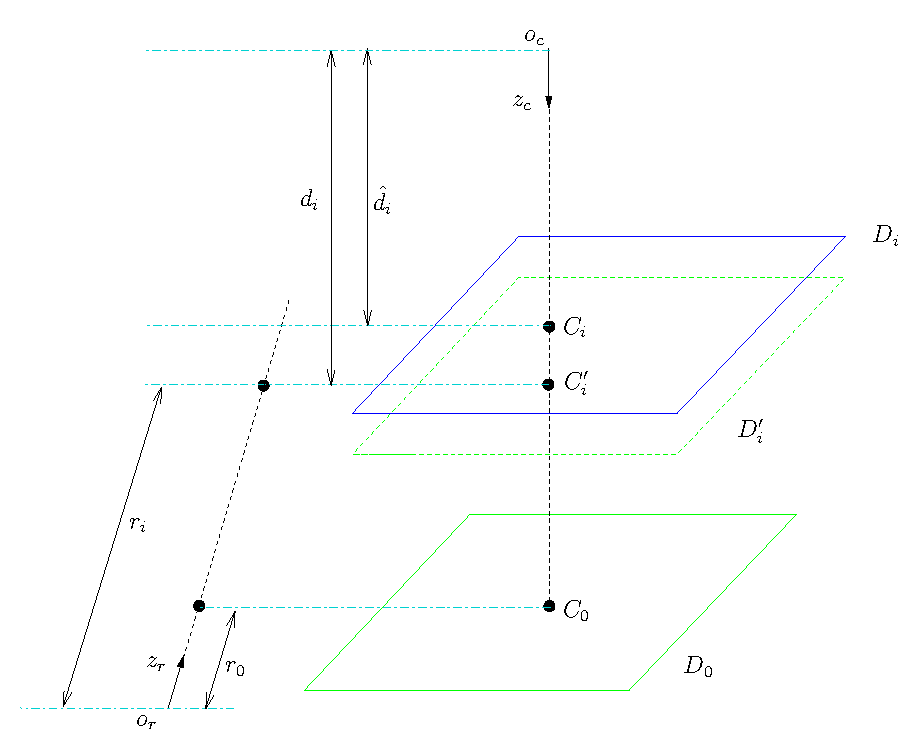
\includegraphics[width=10cm]{depth_exp_precision}
  \caption{精度测量原理图}
  \label{fig:depth_exp_precision}
\end{figure}
$\hat{d}_i$的计算相对简单,根据$D_i$中拟合出相机坐标系下平板的平面方程的参数$\Theta_i$,容易得到
\begin{equation}
  \hat{d}_i = -\frac{\theta_i(4)}{\theta_i(3)}
\end{equation}
为了获得实际平板的与相机坐标系的原点的距离,首先以$D_0$平面为基准,将其沿机器人坐标系$z$轴方向移动$r_i-r_0$,得到新的平面方程$\theta'_i$,则
\begin{equation}
  d_i = -\frac{\theta_i'(4)}{\theta_i'(3)}
\end{equation}
% @improve: equations above can be more specific.

\emph{噪声}定义为平板闭合区域内点距离平面拟合方程的距离的均方根(RMS):
\begin{equation}
  Noise_i = \sqrt{\frac{1}{J}\sum_{j=1}^J{\delta_j^2}}
\end{equation}
其中$\delta_j$为点到拟合平面的距离。

\subsection{实验结果}
实验分别对SR300和对偶RGB-D相机在平板距离相机0.2到1.2m范围内采集了$1 + 10$组数据,测得每组数据深度信息的三个指标,填充率随距离变换的曲线如图\ref{fig:fillrate_exp_res}所示。
\begin{figure}[ht]
  \centering
  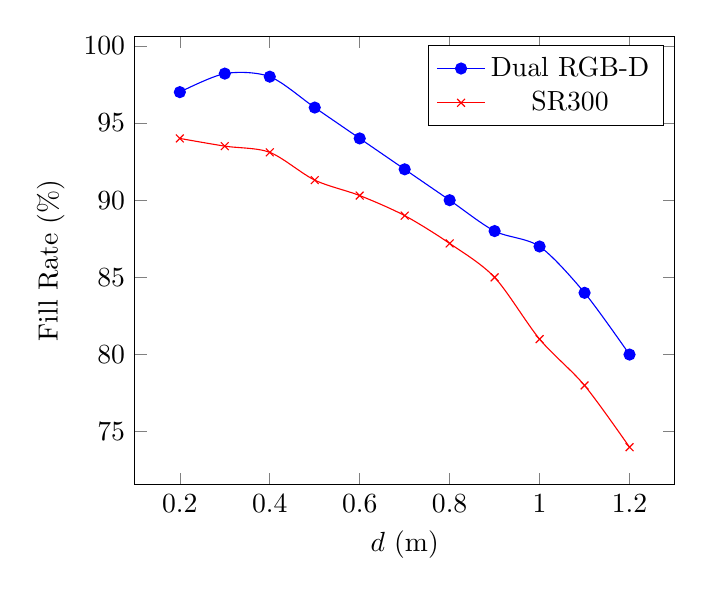
\begin{tikzpicture}
    \begin{axis}[xlabel=$d$ (m), ylabel=Fill Rate (\%)]
      \addplot[smooth, mark=*, blue] plot coordinates {
        (0.2, 97)
        (0.3, 98.2)
        (0.4, 98)
        (0.5, 96)
        (0.6, 94)
        (0.7, 92)
        (0.8, 90)
        (0.9, 88)
        (1.0, 87)
        (1.1, 84)
        (1.2, 80)
      };
      \addlegendentry{Dual RGB-D}
      \addplot[smooth, mark=x, red] plot coordinates {
        (0.2, 94)
        (0.3, 93.5)
        (0.4, 93.1)
        (0.5, 91.3)
        (0.6, 90.3)
        (0.7, 89)
        (0.8, 87.2)
        (0.9, 85)
        (1.0, 81)
        (1.1, 78)
        (1.2, 74)
      };
      \addlegendentry{SR300}
    \end{axis}
  \end{tikzpicture}
  \caption{填充率随距离变化曲线}
  \label{fig:fillrate}
\end{figure}
从图中可以看出随着距离的增加,两个相机的填充率都有所下降,对偶RGB-D相机的填充率相比单个RGB-D相机具有更高的填充率。

深度图的精度随距离的变换曲线如图\ref{fig:precision}所示,从图中可以看出精度在$d=0.4m$处最高,当$d>0.4$时,越远离相机精度越低;当$d<0.4$时,越靠近相机精度越低。对偶RGB-D相机与单个RGB-D相机在精度上略有提升,但提升不大。
\begin{figure}[ht]
  \centering
  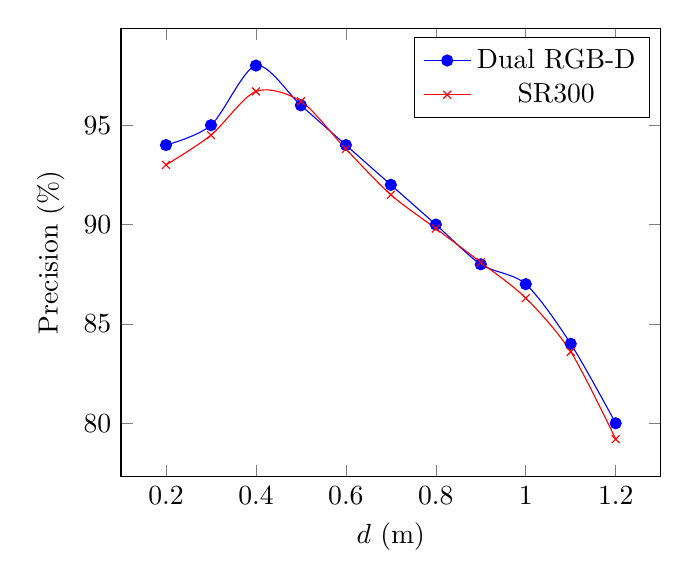
\begin{tikzpicture}
    \begin{axis}[xlabel=$d$ (m), ylabel=Precision (\%)]
      \addplot[smooth, mark=*, blue] plot coordinates {
        (0.2, 94)
        (0.3, 95)
        (0.4, 98)
        (0.5, 96)
        (0.6, 94)
        (0.7, 92)
        (0.8, 90)
        (0.9, 88)
        (1.0, 87)
        (1.1, 84)
        (1.2, 80)
      };
      \addlegendentry{Dual RGB-D}
      \addplot[smooth, mark=x, red] plot coordinates {
        (0.2, 93)
        (0.3, 94.5)
        (0.4, 96.7)
        (0.5, 96.2)
        (0.6, 93.8)
        (0.7, 91.5)
        (0.8, 89.8)
        (0.9, 88.1)
        (1.0, 86.3)
        (1.1, 83.6)
        (1.2, 79.2)
      };
      \addlegendentry{SR300}
    \end{axis}
  \end{tikzpicture}
  \caption{精度随距离变化曲线}
  \label{fig:precision}
\end{figure}

深度信息噪声随距离的变化曲线如图\ref{fig:noise}所示,从图中可以看出噪声随着距离的增加而增加,并且距离越大,噪声增加的越多。在同等距离下,对偶RGB-D相机相比单个RGB-D相机具有更小的噪声。
\begin{figure}[ht]
  \centering
  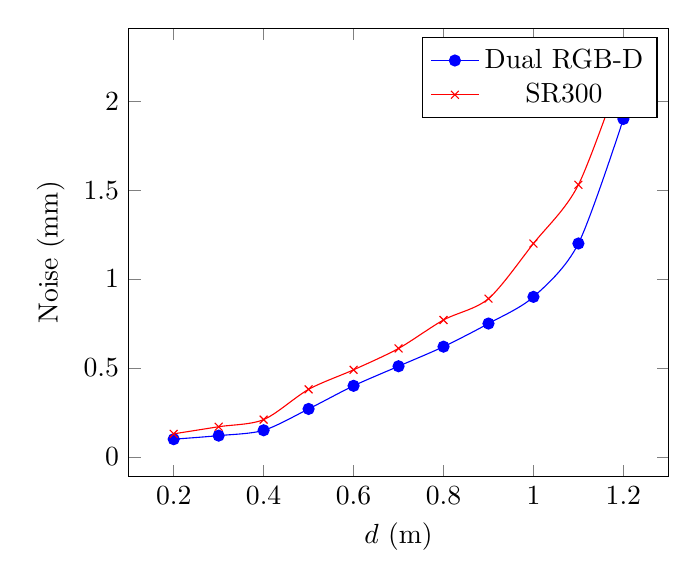
\begin{tikzpicture}
    \begin{axis}[xlabel=$d$ (m), ylabel=Noise (mm)]
      \addplot[smooth, mark=*, blue] plot coordinates {
        (0.2, 0.1)
        (0.3, 0.12)
        (0.4, 0.15)
        (0.5, 0.27)
        (0.6, 0.4)
        (0.7, 0.51)
        (0.8, 0.62)
        (0.9, 0.75)
        (1.0, 0.9)
        (1.1, 1.2)
        (1.2, 1.9)
      };
      \addlegendentry{Dual RGB-D}
      \addplot[smooth, mark=x, red] plot coordinates {
        (0.2, 0.13)
        (0.3, 0.17)
        (0.4, 0.21)
        (0.5, 0.38)
        (0.6, 0.49)
        (0.7, 0.61)
        (0.8, 0.77)
        (0.9, 0.89)
        (1.0, 1.2)
        (1.1, 1.53)
        (1.2, 2.2)
      };
      \addlegendentry{SR300}
    \end{axis}
  \end{tikzpicture}
  \caption{噪声随距离变化曲线}
  \label{fig:noise}
\end{figure}

综上,所设计的对偶RGB-D相机相比SR300相机有更高的填充率,与设计时的初衷一致,毕竟结合了两个相机的深度信息,理论上深度信息的填充率就应该有所增加;对偶RGB-D相机的精度与SR300相机相比没有太显著的提升,但噪声有着明显的下降。综上可以得出对偶RGB-D相机所采集的深度图相比单个RGB-D相机有着更高的填充率、更低的噪声,深度图的质量更好。

\section{本章小结}
本章首先介绍了RGB-D相机的现状,然后详细介绍了以结构光为原理的RGB-D相机SR300的原理以及标定方法,针对SR300对于反光物体深度信息缺失的情况,通过组合两个RGB-D相机构成对偶RGB-D相机实现采集高质量的深度图,并给出了对偶RGB-D相机的标定流程。最后设计了深度图质量测试的实验,证明了对偶RGB-D相机比单个RGB-D相机有更高的填充率,更低的噪声。

%%% Local Variables:
%%% mode: latex
%%% TeX-master: "../thesis"
%%% End:
